\chapter{Vision}


This chapter covers the transformation of 2D stereo images into a useful 3D point cloud. Using only a stereo camera as passive sensor.

\section{Theory - Dense Stereo}

Dense stereo uses two 2D images and converts them to a dense 3D point cloud. That is the 3D postion of every point in the 2D images is desired. To obtain this the disparity between all features are required, and the following stages are done with that in mind. The stages are as following.

\begin{itemize}
  \item Undistortion
  \item Rectification
  \item Correspondence
  \item Reprojection
\end{itemize}


\subsection{Undistortion and Rectification}


The undistortion and rectification is performed automatically and therefore only a short description will be included. By knowledge of these parameters one could make functions take them into account, but it is much more effective to transform the images.

As a lense is used for the cameras the normal camera model cannot be used, i.e. a 3D point, X, is mapped to the image plane, x, by $ x = f X/Z $, where f is the focal length and Z is the distance to the camera. Both radial and tangential distortion exist respectively creating the circular and elliptical distortion. By correcting the image for these parameters all pixels now follow the camera model and their projection line can be found.

The basic idea of rectification is based on epipolar lines. Epipolar lines are created by knowing the transform between the cameras. For every single point in one camera the line on which it can appear on another camera can be found. That is the epipolar line is a mapping of a pixels projection line in one camera to onto the image plane of another camera. 

By knowing the transformation between the two images, epipolar lines can be created for every point. An epipolar line is the line on which any point in one image must be positioned in the other image. Thus making the search for a feature much faster as it only occurs in one dimension.

Rectification takes this one step further. By rectifying the two images the camera planes are made to be parallel. Making the search for correspondence a one dimensional, horizontal task, drastically increasing the speed.

% 

Thus undistortion is a manipulation done independently for the cameras and the rectification is performed for the two cameras together, respectively an intrinsic and extrinsic parameter.


%Normally when modelling a camera the pinhole model is used, i.g. a 3D point, X, is mapped to the image plane, x, by $ x = f X/Z $, where f is the focal length and Z is the distance to the camera. Though a camera with a single pinhole would have a very long shutter time to gather enough light for an image. Thus to decrease shutter time a lens is used to concentrate more light on the image sensor. But as the lens is not perfect the image no longer complies with the pinhole camera model. By undistorting the images the actual projection point can be found for the images. 
%
%\subsubsection{Radial}
%
%The radial distortion appears as the lens is not perfectly parabolic, but spherical. That is expressed by an increasing distortion of the image the further one gets from the center of the image. 
%
%\[x = x(1 + k_{1} r^{2} + k_{2}^{4} + k_{3}^{6} ) \ldots \] 
%\[y = y(1 + k_{1} r^{2} + k_{2}^{4} + k_{3}^{6} ) \ldots \]
%
%
%\subsubsection{Tangential}
%
%The tangential distortion appears because of a misalignment between the center of the lens and the center of the sensor. Thus the circular distortion appears elliptical and further distortion parameters are needed.
%
%\[x = x + [2p_{1}y + p_{2}(r^{2} + 2x^{2} ) \ldots  ] \] 
%
%\[y = x + [p_{1}(r^{2} + 2y^{2} ) + 2p_{2}x \ldots ] \] 
%
%\subsection{Rectification}
%
%To find the 3D position of a point it's position must be known in both images. That is a matching between pixels must be performed for the two images. Rectification is a process which not only speeds up this process, but also increases accuracy.
%
%The idea is based on epipolar lines. Epipolar lines are created by knowing the transform between the cameras. For every single point in one camera the line on which it can appear on another camera can be found. The reason that this epipolar line exist is that though the actual 3D position of a projection line for the point can be found. That is the linear connection between X and Z in the camera matrix. Thus by the transform matrix the projection line can be projected into an epipolar line in an other camera.  
%
%By knowing the transformation between the two images, epipolar lines can be created for every point. An epipolar line is the line on which any point in one image must be positioned in the other image. Thus making the search for a feature much faster as it only occurs in one dimension.
%
%Rectification takes this one step further. By rectifying the two images the camera planes are made to be parallel. Making the search for correspondence a one dimensional horizontal endeavour, drastically increasing the speed.
%
%Thus undistortion is a manipulation done independently for the cameras and the rectification is performed for the two cameras together.
%
%""" matrixer """

\subsection{Correspondence} \label{sec:correspondence}

Correspondence is the matching between position of pixels in the two images. This creates a disparity map for all pixels in the two images. Though only if a proper match can be performed.

The matching can be done with either a single pixel or larger pixel patches.

Simple, dynamic, global.

The method used is the Semi-Global block matching.

\[ E(D) = \sum\limits_{p}(C(p,D_{p}) + \sum\limits_{q \in N_{p} } P_{1} T [|D_{p} - D_{q}| = 1] + \sum\limits_{q \in N_{p} } P_{2} T [|D_{p} - D_{q}| > 1] \]

Global matching tries to minimize the overall error in the disparity image. That is creating the optimal disparity image, though this is an NP-hard problem and thus more local approaches are implemented. 

The most simple is the one would be a simple linear search.

\subsection{Reprojection} \label{sec:reprojection}

During the calibration of the cameras, projections matrices were obtained for both cameras. The projection matrices are based on the left camera lens, meaning the baseline, distance to the left camera, is 0 for the left matrix. By multiplying the projection matrix with a 3D point in the left cameras  compared to the left camera, the points position in the image can be found. That is:

\[ 
\begin{pmatrix}
  x \\
  y \\
  \omega 
 \end{pmatrix}	
 = 
 \begin{pmatrix}
  F_{x} & 0 & C_{x} & -F_{x}T_{x} \\
  0 & F_{y} & C_{y} & 0 \\
  0 & 0 & 1 & 0
 \end{pmatrix}
 \begin{pmatrix}
  X \\
  Y \\
  Z \\
  1 
 \end{pmatrix}	
\]

Here $F_{x}$ and $F_{y}$ are the focal length of the camera, $C_{x}$ and $C_{y}$ are the middle position of the image.

$T_{x}$ is the translation to the left camera. That is for the right camera it is the baseline and for the left it is 0. The baseline is measured in millimetres. 

But goal is to obtain the opposite, the transform from 2D to 3D. That is the action of converting the obtained disparity map into a 3D point cloud. To do that the x and y positions are combined with the disparity. Thus multiplying with the Q matrix the 3D map position can be found.

\[ Q [ x \ y \ d \ 1 ]^{T} = [ X \ Y \ Z \ W ]^{T} \]

Where the Q matrix is defined by the right projection matrix, except for the $C_{x}'$.

\[
Q =
 \begin{pmatrix}
  1 & 0 & 0 & -C_{x} \\
  0 & 1 & 0 & -C_{y} \\
  0 & 0 & 0 & F_{x} \\
  0 & 0 & -1/T_{x} & (C_{x}-C_{x}')/T_{x} 
 \end{pmatrix}
\]

Thus multiplying with the above mentioned vector, and scaling W to zero the 3D position can be obtained.

\[
 \begin{pmatrix}
  x - C_{x} \\
  y - C_{y} \\
  F_{x} \\
  d-1/T_{x} 
 \end{pmatrix}
 \Rightarrow
  \begin{pmatrix}  
  X\\
  Y\\
  Z
 \end{pmatrix}
 =
 \begin{pmatrix}
  \dfrac{x - C_{x}}{ d(-1/T_{x})}  \\
  \dfrac{y - C_{y} }{ d(-1/T_{x})}\\
  \dfrac{F_{x}}{ d(-1/T_{x})}\\
  1
 \end{pmatrix}
\]

\section{Method - Images to point cloud}

As the project uses ROS for communication between nodes as much as possible ROS have been used for the stereo operations. Though it wasn't possible to use generic ROS nodes for every operation, the reason for this is explained in section \ref{sec:optimizing_parameters}. 

\subsection{Calibration} \label{sec:calibration}

To perform the undistortion and rectification the intrinsic and extrinsic parameters of the cameras are required. These were obtained by the ROS node $stereo\_camera\_calibrate$ by capturing images of a known chessboard pattern in different positions and rotations. When enough images have been captured the ROS node have enough input to solve for the camera parameters. It thus returns the camera matrix along with distortion parameters and the distance between the cameras.

% A small calibration plate were used, so that the calibration could be done within a meter from camera, fitting the parameters for the specific task.

\subsection{Undistortion and rectification}

Undistortion and rectification is done with a simple ROS node called image $image\_proc$. By setting giving the raw images together with a camera calibration file, created beforehand in section \ref{sec:calibration}. It uses these and returns rectified and undistorted images ready to be used by block matching algorithms.

\subsection{Blockmatching and reprojection}

The blockmatching is done with the OpenCV function SGBM described in section \ref{sec:correspondence}. Time stamps are checked for arriving images to make sure that they are recorded at the same time. The SGBM then uses the images and a certain set of parameters, discussed in section \ref{sec:optimizing_parameters} to make a disparity map. Conversion from int16 to float32 by division of 16.


A ROS node is created takes the rectified images, creates a disparity map and reprojects this to 3D using OpenCV functions.

\section{Results}

Here results from the different operations are shown, these results are qualitative to show that the concept works not quantitative for a measurement of how well.

\subsection{Calibration}

From the calibration, the both the distortion parameters and the projection matrixes are returned. The distortion parameters can be seen in equation \ref{eq:distortion}. An example of using these values for undistortion can be seen in image \ref{fig:undistorted}.

label figure   Example of the undistortion.


\begin{equation}\label{eq:distortion}
\begin{split}
[ k_{1}, k_{2}, p_{1}, p_{2}, k_{3} ] = [\ -0.422868,\ 0.192589,\ -0.000004,\ 0.002985,\ 0.000000\ ]
\end{split}
\end{equation} 

The rotation matrix for rectification are also returned from the calibration. It can be seen that the rotation needed is small but still needed for the 1D correspondence to work. 

\begin{equation}\label{eq:distortion}
\begin{split}
R =
 \begin{pmatrix}
  0.998701 & -0.002701 & -0.050892 \\
  0.002645 & 0.999996 & -0.001179 \\
  0.050895 & 0.001043 & 0.998703 
 \end{pmatrix}
\end{split}
\end{equation}

Figure \ref{fig:rectified} shows and example of two output images from $image\_proc$. These images are both undistorted and rectified by the function. The image have included horizontal lines showing the effectiveness of the image to align features.

\begin{figure}[h!]
  \caption{Result of undistortion and rectification on an image pair. The horizontal lines shows corresponding pixels in the two images.}
  \centering
    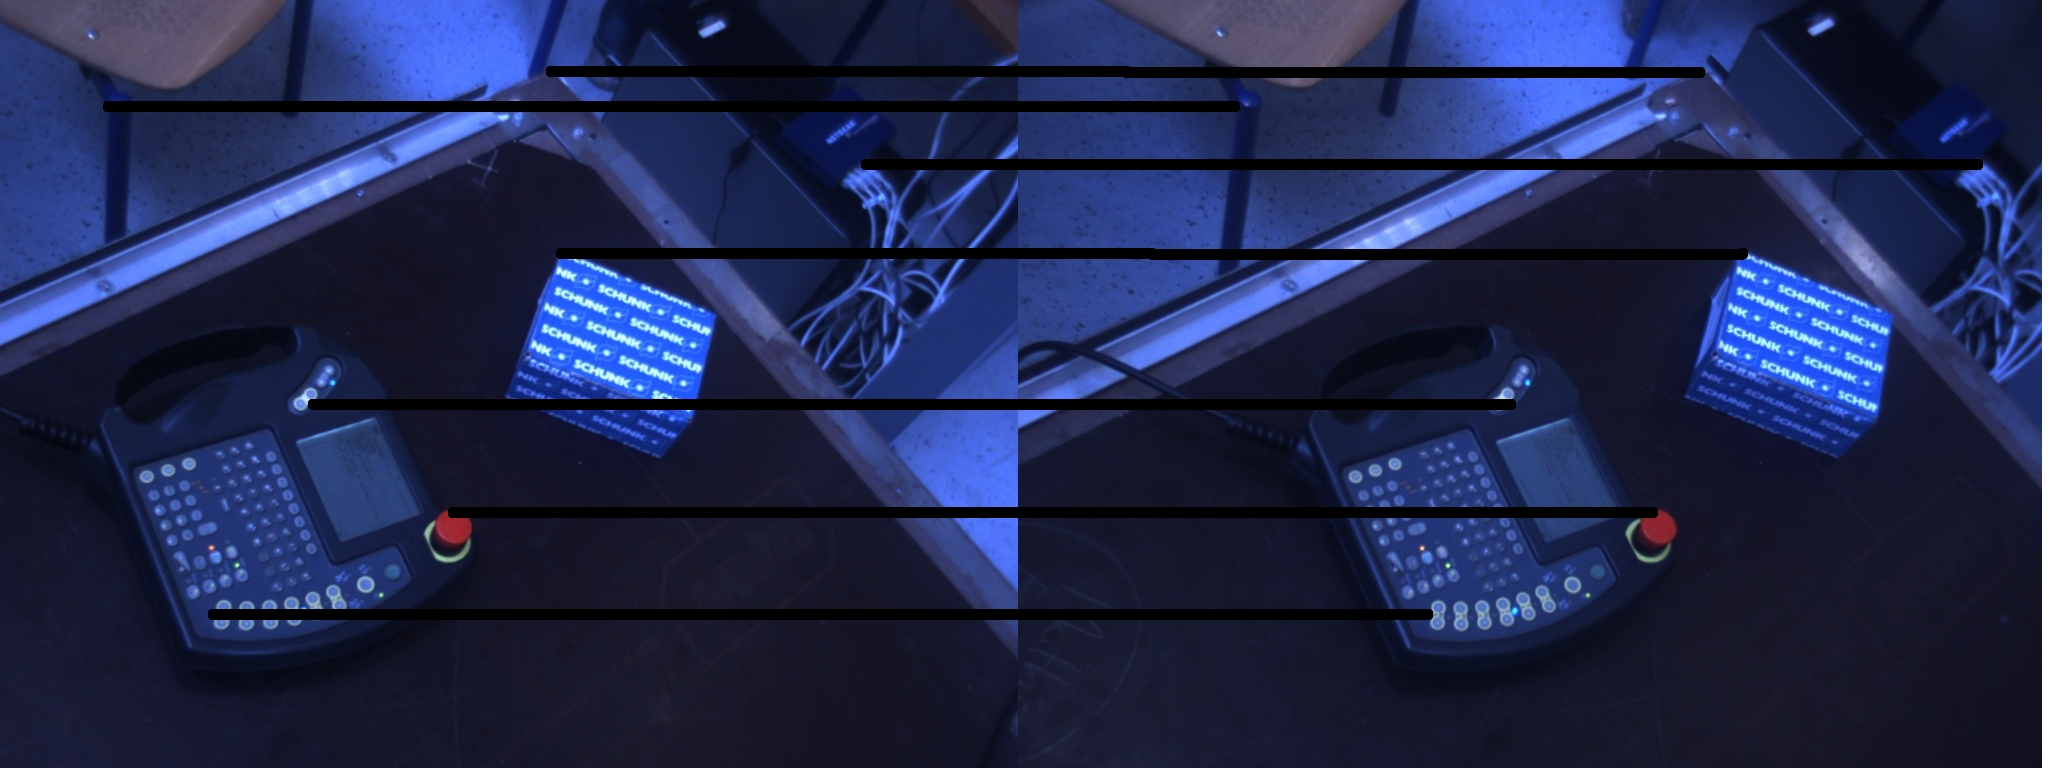
\includegraphics[width=\textwidth]{graphics/06_vision/rectified.jpg}
    \label{fig:rectified}
\end{figure}

\subsection{Disparity map}

From two rectified images the disparity map can be created. Figure \ref{fig:disparity} is an example of such a disparity map. The overall structure of the scene is recognizable, but it can be seen that algorithm does not necessarily guarantees complete coverage with standard parameters. Thus section \ref{sec:optimizing_parameters} will include a discussion of the selection of these parameters.

\begin{figure}[h!]
  \caption{Disparity image for the two images shown in figure \ref{fig:rectified}. }
  \centering
    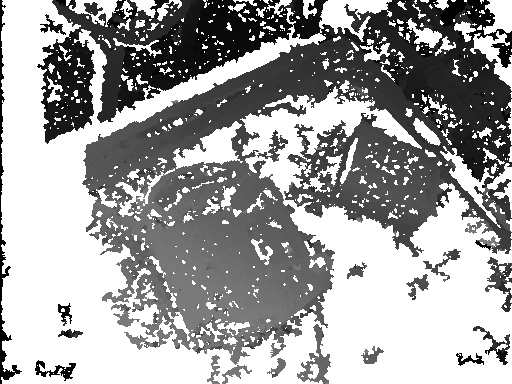
\includegraphics[scale=0.4]{graphics/06_vision/disparity_example.jpg}
    \label{fig:disparity}
\end{figure}


\subsection{Reprojected point clouds} \label{sec:repro_point}

The only thing left to do is reprojecting the disparity map into 3D coordinates. From the calibration the parameters in \ref{eq:parameters} were given for the right camera.

\begin{equation}\label{eq:parameters}
\begin{split}
Cx = 582.152313 \\
Cy = 393.397633 \\
Fx = 1321.556521 \\
????? = 158.751707 
\end{split}
\end{equation} 

Given  ?????  the baseline between the cameras calculated as in equation \ref{eq:baseline}.

\begin{equation}\label{eq:baseline}
\begin{split}
Tx = ?????/(-Fx) = Tx = 158.8/-1321.6 = 0.1201 meters
\end{split}
\end{equation} 

Using these parameters in the Q-matrix the disparity image is reprojected to 3D. An example of the reprojection for the disparity image in figure \ref{fig:disparity} can be seen in figure \ref{fig:repro_point}


\begin{figure}[h!]
  \caption{Point cloud reprojected using the parameters shown in section \ref{sec:repro_point} performed on the disparity image in figure \ref{fig:repro_point}. }
  \centering
    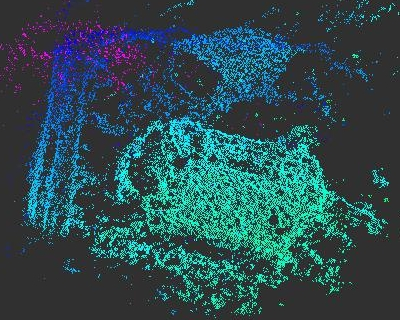
\includegraphics[scale=0.7]{graphics/06_vision/point_cloud_example2.jpg} %trim=l b r t
    \label{fig:point_repro}
\end{figure}


\section{ Optimizing parameters towards the task } \label{sec:optimizing_parameters}

In most of the functions the input were non-adjustable values, but for the SGBM there are certain parameters were no single answers exist. The most important being the disparity range i.e. how far the algorithm will search for 


When the 3D positions were extracted in section \ref{sec:reprojection} the connection in equation \ref{eq:disp1} between distance and disparity were found.

\begin{equation}\label{eq:disp1}
\begin{split}
Z = \dfrac{F_{x}}{ d(-1/T_{x})}
\end{split}
\end{equation} 

When solving for disparity the connection in equation \ref{eq:disp2} is given.

\begin{equation}\label{eq:disp2}
\begin{split}
 d = \dfrac{F_{x}T_{x}}{ Z}
\end{split}
\end{equation} 

That is with a known distance to the setup the one knows the search area, and thus the disparity range can also be calculated. Thus the distance is around 0.5 meters and the focal length and baseline is known from the calibration and shown in section \ref{sec:repro_point}. Thus the expected disparity can be calculated as in equation \ref{eq:disp3}.

\begin{equation}\label{eq:disp3}
\begin{split}
d = \dfrac{1321.55 pixel*0.1201m}{0.5m} = 317.4 pixel
\end{split}
\end{equation}

Thus the minimum and maximum disparity both have to range around this number. It is because of this that the point cloud generated from the ROS $image\_proc$ cannot be used. The node is only able to search with a maximum disparity range of 128 pixel. This gives a minimum distance of 1.24 meters. This wouldn't fit the desired setup at all and therefore the automatically generated point cloud is rejected. The exact disparity range can be found by looking at the maximum size of the object. This is an important aspect as setting the correct disparity range will drastically increase the search time and potentially remove mismatches.